% -*- root: ../../main.tex -*- %

\AnhChapter{Theoretical Background}
  \AnhSection{Docker}
    \begin{figure}[htbp]
      \centering
      \begin{tikzpicture}[scale=0.8,->,>=stealth',shorten >=1pt,auto,node distance=5cm, semithick]
        \sffamily\fontsize{10}{10}\selectfont
        \node (cr){};
        \node (run){};
        \node[state] (A)     [right =3cm of cr]         {created};
        \node[state]         (B) [right =2.5cm of A] {running};
        \node[state]         (C) [below right of=B] {stopped};
        \node[state]         (D) [above =2cm of B] {paused};
        \node[state]         (E) [below =2cm of A] {deleted};

        \path (cr) edge [] node {create} (A)
            (run) edge [out=45,in=150]                     node {run} (B)
              (A) edge []                              node {start} (B)
                  edge [bend right]                    node {rm}    (E)
              (B) edge [out=230, in=200, distance=4cm] node {kill}  (C)
                  edge [out=250,in=175, distance=2.5cm]node {stop}  (C)
                  edge [bend left]                     node {pause}  (D)
                  edge [in=30, out=45, loop]           node {restart}  (D)
                  edge [out=10, in=90, distance=2cm]   node {\textit{container process exited}}  (C)
              (C) edge [bend right]                    node {start}  (B)
                  edge [bend left]                     node {rm}  (E)
              (D) edge [bend left]                     node {unpause} (B)
              ;
      \end{tikzpicture}
      \caption*{Simplified version. Commands should be understood prefixed with \texttt{docker}. \newline \scriptsize Based on https://docs.docker.com/engine/reference/api/docker\_remote\_api/\#docker-events }
      \caption[Docker Container Life Cycle]{Docker Container Life Cycle \cite{Docker2016Docker}}
      \label{fig:docker_container_lifecycle}
    \end{figure}
\clearpage
\AnhChapter{Architecture and design}

  % \begin{figure}[htbp]
  %   \centering
  %   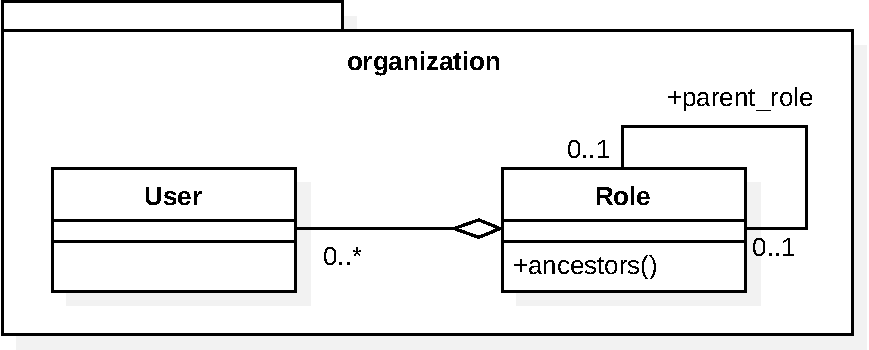
\includegraphics[width=0.65\textwidth]{content/images/class_diagram_organization-crop.pdf}
  %   \caption{UML class diagram for the organization service}
  % \label{fig:uml_class_diagram_organization}
  % \end{figure}

  \begin{figure}[htbp]
    \centering
    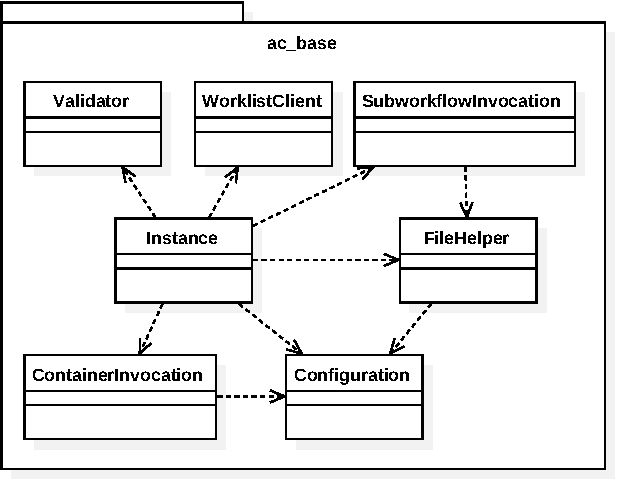
\includegraphics[width=0.65\textwidth]{content/images/class_diagram_activity_image-crop.pdf}
    \caption{UML class diagram for the activity image}
  \label{fig:uml_class_diagram_ac_base}
  \end{figure}

  \begin{figure}[htbp]
    \centering
    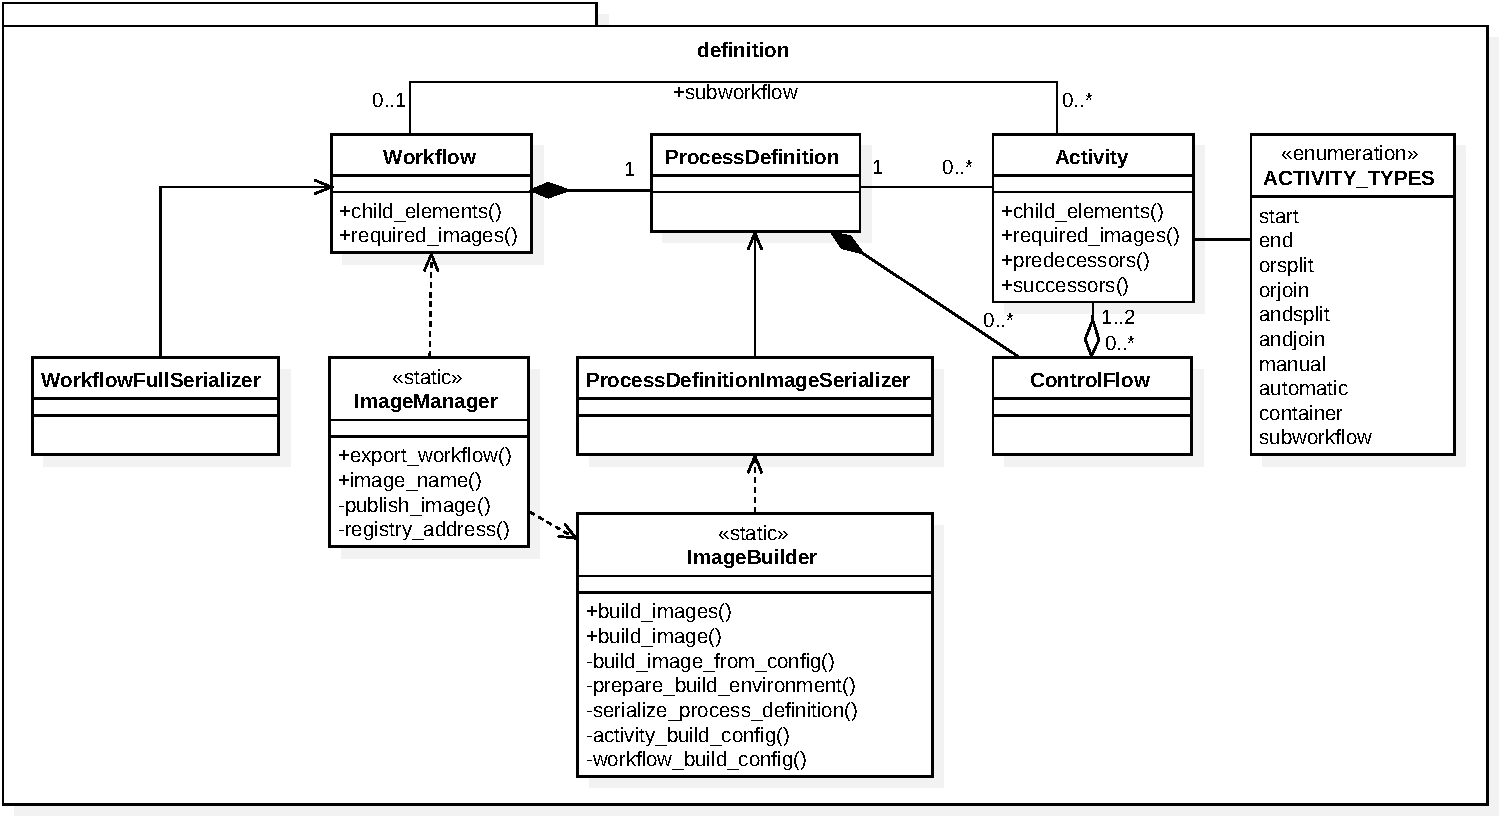
\includegraphics[width=0.95\textwidth]{content/images/class_diagram_definition-crop.pdf}
    \caption{UML class diagram for the definition service}
    \label{fig:class_diagram_definition}
  \end{figure}

  \begin{figure}[htbp]
    \centering
    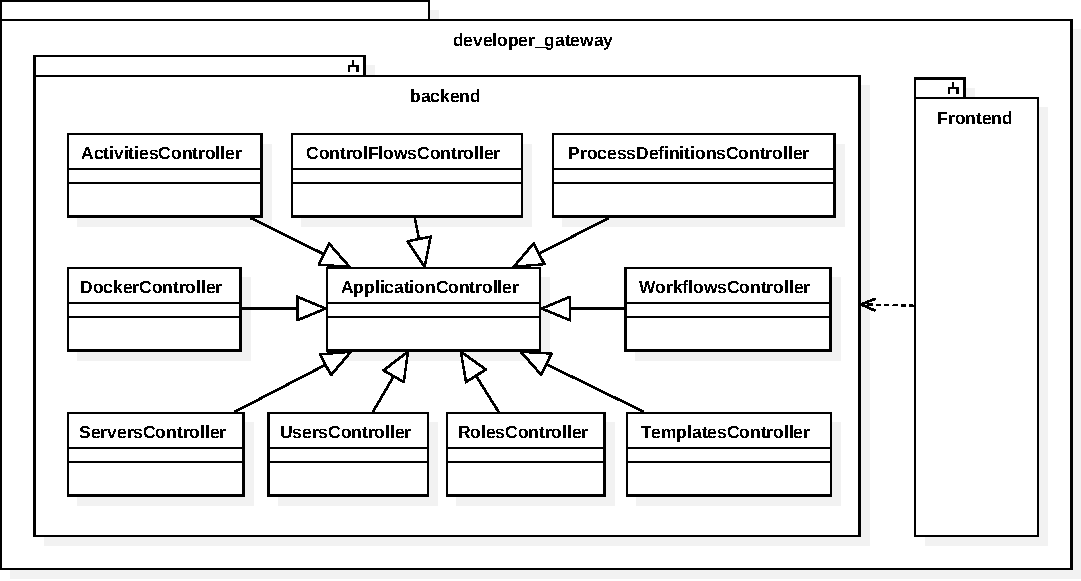
\includegraphics[width=0.95\textwidth]{content/images/class_diagram_developer_gateway-crop.pdf}
    \caption{UML class diagram for the developer gateway}
    \label{fig:class_diagram_developer_gateway}
  \end{figure}

  \begin{figure}[htbp]
    \centering
    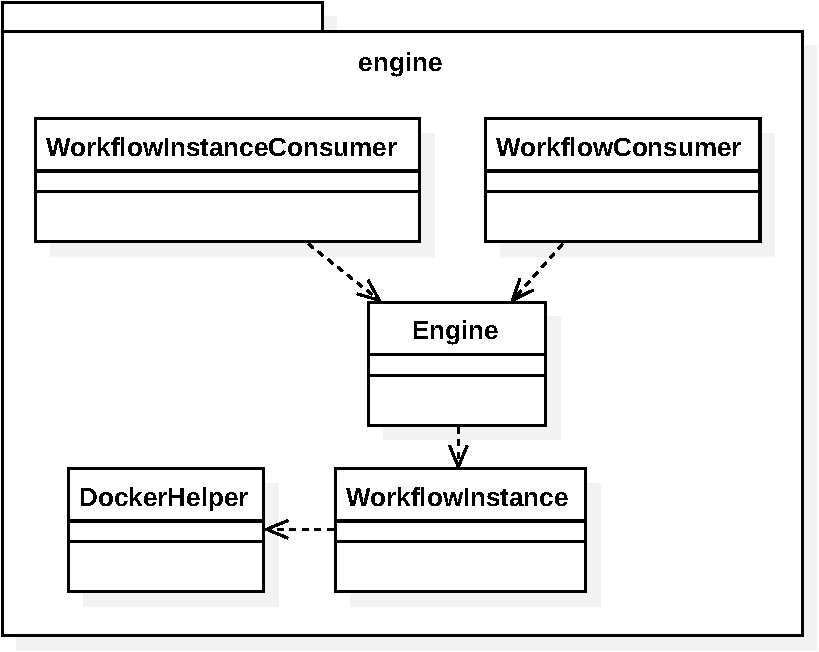
\includegraphics[width=0.65\textwidth]{content/images/class_diagram_engine-crop.pdf}
    \caption{UML class diagram for the workflow engine service}
    \label{fig:class_diagram_engine}
  \end{figure}

  \begin{figure}[htbp]
    \centering
    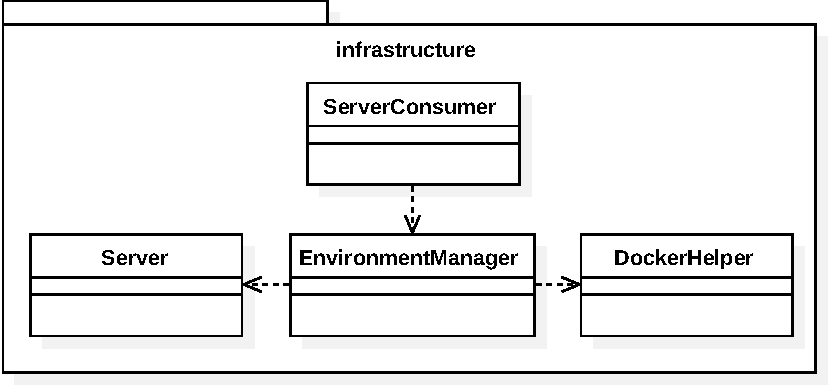
\includegraphics[width=0.65\textwidth]{content/images/class_diagram_infrastructure-crop.pdf}
    \caption{UML class diagram the infrastructure management service}
    \label{fig:class_diagram_infrastructure}
  \end{figure}

  \begin{figure}[htbp]
    \centering
    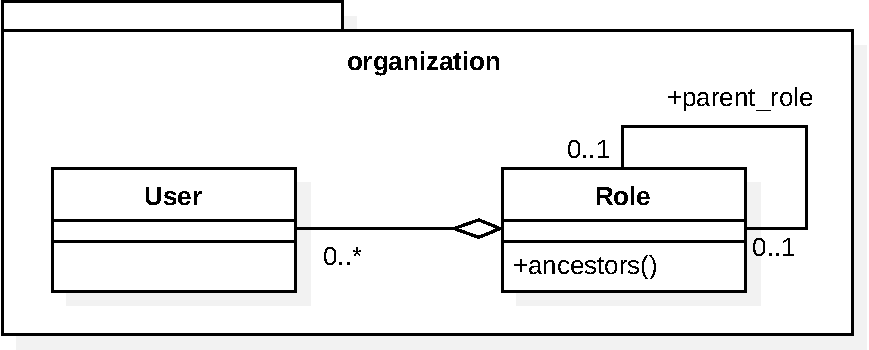
\includegraphics[width=0.65\textwidth]{content/images/class_diagram_organization-crop.pdf}
    \caption{UML class diagram the organization management service}
    \label{fig:class_diagram_organization}
  \end{figure}

  \begin{figure}[htbp]
    \centering
    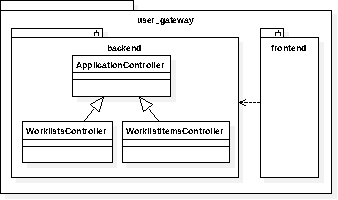
\includegraphics[width=0.65\textwidth]{content/images/class_diagram_user_gateway-crop.pdf}
    \caption{UML class diagram the user gateway}
    \label{fig:class_diagram_user_gateway}
  \end{figure}

  \begin{figure}[htbp]
    \centering
    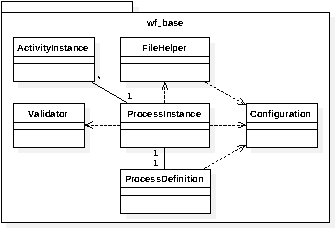
\includegraphics[width=0.65\textwidth]{content/images/class_diagram_wf_base-crop.pdf}
    \caption{UML class diagram the workflow image}
    \label{fig:class_diagram_wf_base}
  \end{figure}

  \begin{figure}[htbp]
    \centering
    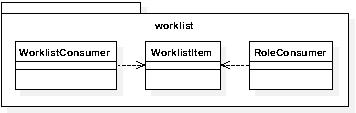
\includegraphics[width=0.65\textwidth]{content/images/class_diagram_worklist-crop.pdf}
    \caption{UML class diagram the worklist service}
    \label{fig:class_diagram_worklist}
  \end{figure}

 \clearpage
\AnhChapter{Implementation}
  \AnhSection{Workflow image}

    \begin{listing}[!h]
      \inputminted[fontsize=\footnotesize,linenos=true,numberblanklines=true,showspaces=false,breaklines=true,baselinestretch=1]{json}{./content/snippets/process_definition.json}
      \caption{Exported process definition in JSON format}
    \label{lst:exported_process_definition_in_json_format}
    \end{listing}

    \begin{listing}[!h]
      \inputminted[fontsize=\footnotesize,linenos=true,numberblanklines=true,showspaces=false,breaklines=true,baselinestretch=1]{json}{./content/snippets/wf_image/input.schema.json}
      \caption*{ \mintinline{json}| {"this":"is a test"} | would be considered valid input data with the depicted schema }
      \caption{JSON schema used for input validation}
    \label{lst:input_schema_in_json_format}
    \end{listing}

    \begin{listing}[!h]
      \inputminted[fontsize=\footnotesize,linenos=true,numberblanklines=true,showspaces=false,breaklines=true,baselinestretch=1]{Dockerfile}{../code/wf_base/Dockerfile}
      \caption{Dockerfile for workflow base image}
    \label{lst:dockerfile_for_workflow_base_image}
    \end{listing}

    \begin{listing}[!h]
      \inputminted[lastline=39,fontsize=\footnotesize,linenos=true,numberblanklines=true,showspaces=false,breaklines=true,baselinestretch=1]{ruby}{../code/wf_base/activity_instance.rb}
      \caption{ActivityInstance class in workflow image (1/2)}
    \label{lst:wf_image_activity_instance}
    \end{listing}

    \begin{listing}[!h]
      \inputminted[firstline=40,fontsize=\footnotesize,linenos=true,numberblanklines=true,showspaces=false,breaklines=true,baselinestretch=1]{ruby}{../code/wf_base/activity_instance.rb}
      \caption{ActivityInstance class in workflow image (2/2)}
    \label{lst:wf_image_activity_instance_2}
    \end{listing}

    \begin{listing}[!h]
      \inputminted[lastline=49,fontsize=\footnotesize,linenos=true,numberblanklines=true,showspaces=false,breaklines=true,baselinestretch=1]{ruby}{../code/wf_base/file_helper.rb}
      \caption{FileHelper helper class in workflow image (1/2)}
    \label{lst:wf_image_file_helper}
    \end{listing}

    \begin{listing}[!h]
      \inputminted[firstline=50,fontsize=\footnotesize,linenos=true,numberblanklines=true,showspaces=false,breaklines=true,baselinestretch=1]{ruby}{../code/wf_base/file_helper.rb}
      \caption{FileHelper helper class in workflow image (2/2)}
    \label{lst:wf_image_file_helper_2}
    \end{listing}

    \begin{listing}[!h]
      \inputminted[lastline=43,fontsize=\footnotesize,linenos=true,numberblanklines=true,showspaces=false,breaklines=true,baselinestretch=1]{ruby}{../code/wf_base/process_definition.rb}
      \caption{ProcessDefinition class in workflow image (1/2)}
    \label{lst:wf_image_process_definition}
    \end{listing}

    \begin{listing}[!h]
      \inputminted[firstline=44,fontsize=\footnotesize,linenos=true,numberblanklines=true,showspaces=false,breaklines=true,baselinestretch=1]{ruby}{../code/wf_base/process_definition.rb}
      \caption{ProcessDefinition class in workflow image (2/2)}
    \label{lst:wf_image_process_definition_2}
    \end{listing}

    \begin{listing}[!h]
      \inputminted[lastline=45,fontsize=\footnotesize,linenos=true,numberblanklines=true,showspaces=false,breaklines=true,baselinestretch=1]{ruby}{../code/wf_base/process_instance.rb}
      \caption{ProcessInstance class in workflow image (1/2)}
    \label{lst:wf_image_process_instance}
    \end{listing}

    \begin{listing}[!h]
      \inputminted[firstline=46,fontsize=\footnotesize,linenos=true,numberblanklines=true,showspaces=false,breaklines=true,baselinestretch=1]{ruby}{../code/wf_base/process_instance.rb}
      \caption{ProcessInstance class in workflow image (2/2)}
    \label{lst:wf_image_process_instance_2}
    \end{listing}

    \begin{listing}[!h]
      \inputminted[fontsize=\footnotesize,linenos=true,numberblanklines=true,showspaces=false,breaklines=true,baselinestretch=1]{ruby}{../code/wf_base/run.rb}
      \caption{Workflow image run script}
    \label{lst:wf_image_run}
    \end{listing}

  \clearpage
  \AnhSection{Activity image}

    \begin{listing}[!h]
      \inputminted[fontsize=\footnotesize,linenos=true,numberblanklines=true,showspaces=false,breaklines=true,baselinestretch=1]{Dockerfile}{../code/ac_base/Dockerfile}
      \caption{Dockerfile for activity base image}
    \label{lst:dockerfile_for_activity_base_image}
    \end{listing}

    \begin{listing}[!h]
      \inputminted[firstline=8,lastline=58,fontsize=\footnotesize,linenos=true,numberblanklines=true,showspaces=false,breaklines=true,baselinestretch=1]{ruby}{../code/ac_base/run.rb}
      \caption{Activity instance class (1/2)}
    \label{lst:activity_instance_class}
    \end{listing}

    \begin{listing}[!h]
      \inputminted[firstline=59,fontsize=\footnotesize,linenos=true,numberblanklines=true,showspaces=false,breaklines=true,baselinestretch=1]{ruby}{../code/ac_base/run.rb}
      \caption{Activity instance class (2/2)}
    \label{lst:activity_instance_class_2}
    \end{listing}

    \begin{listing}[!h]
      \inputminted[fontsize=\footnotesize,linenos=true,numberblanklines=true,showspaces=false,breaklines=true,baselinestretch=1]{ruby}{../code/ac_base/container_invocation.rb}
      \caption{ContainerInvocation helper class}
    \label{lst:container_invocation_helper_class}
    \end{listing}

    \begin{listing}[!h]
      \inputminted[lastline=42,fontsize=\footnotesize,linenos=true,numberblanklines=true,showspaces=false,breaklines=true,baselinestretch=1]{ruby}{../code/ac_base/subworkflow_invocation.rb}
      \caption{SubworkflowInvocation helper class (1/2)}
    \label{lst:subworkflow_invocation_helper_class}
    \end{listing}

    \begin{listing}[!h]
      \inputminted[firstline=43,fontsize=\footnotesize,linenos=true,numberblanklines=true,showspaces=false,breaklines=true,baselinestretch=1]{ruby}{../code/ac_base/subworkflow_invocation.rb}
      \caption{SubworkflowInvocation helper class (2/2)}
    \label{lst:subworkflow_invocation_helper_class_2}
    \end{listing}

    \begin{listing}[!h]
      \inputminted[lastline=53,fontsize=\footnotesize,linenos=true,numberblanklines=true,showspaces=false,breaklines=true,baselinestretch=1]{ruby}{../code/ac_base/worklist_client.rb}
      \caption{WorklistClient class (1/2)}
    \label{lst:worklist_client_class}
    \end{listing}

    \begin{listing}[!h]
      \inputminted[firstline=54,fontsize=\footnotesize,linenos=true,numberblanklines=true,showspaces=false,breaklines=true,baselinestretch=1]{ruby}{../code/ac_base/worklist_client.rb}
      \caption{WorklistClient class (2/2)}
    \label{lst:worklist_client_class_2}
    \end{listing}

    \begin{listing}[!h]
      \inputminted[fontsize=\footnotesize,linenos=true,numberblanklines=true,showspaces=false,breaklines=true,baselinestretch=1]{json}{./content/snippets/ac_image/activity.info.json}
      \caption{Activity information for the inclusion in the activity image}
    \label{lst:activity_info_json}
    \end{listing}

  \clearpage
  \AnhSection{Workflow definition service}

    \begin{listing}[!h]
      \inputminted[fontsize=\footnotesize,linenos=true,numberblanklines=true,showspaces=false,breaklines=true,baselinestretch=1]{ruby}{../code/definition/definition.rb}
      \caption{Definition service run script}
    \label{lst:definition_run}
    \end{listing}

    \begin{listing}[!h]
      \inputminted[fontsize=\footnotesize,linenos=true,numberblanklines=true,showspaces=false,breaklines=true,baselinestretch=1]{ruby}{../code/definition/serializers/process_definition_image_serializer.rb}
      \caption{ProcessDefinitionImageSerializer class}
    \label{lst:process_definition_image_serializer}
    \end{listing}

    \begin{listing}[!h]
      \inputminted[fontsize=\footnotesize,linenos=true,numberblanklines=true,showspaces=false,breaklines=true,baselinestretch=1]{ruby}{../code/definition/serializers/workflow_full_serializer.rb}
      \caption{WorkflowFullSerializer class}
    \label{lst:workflow_full_serializer}
    \end{listing}

    \begin{listing}[!h]
      \inputminted[lastline=45,fontsize=\footnotesize,linenos=true,numberblanklines=true,showspaces=false,breaklines=true,baselinestretch=1]{ruby}{../code/definition/models/activity.rb}
      \caption{Activity class (1/2)}
    \label{lst:activity}
    \end{listing}

    \begin{listing}[!h]
      \inputminted[firstline=46,fontsize=\footnotesize,linenos=true,numberblanklines=true,showspaces=false,breaklines=true,baselinestretch=1]{ruby}{../code/definition/models/activity.rb}
      \caption{Activity class (2/2)}
    \label{lst:activity_2}
    \end{listing}

    \begin{listing}[!h]
      \inputminted[fontsize=\footnotesize,linenos=true,numberblanklines=true,showspaces=false,breaklines=true,baselinestretch=1]{ruby}{../code/definition/models/control_flow.rb}
      \caption{ControlFlow class}
    \label{lst:control_flow}
    \end{listing}

    \begin{listing}[!h]
      \inputminted[fontsize=\footnotesize,linenos=true,numberblanklines=true,showspaces=false,breaklines=true,baselinestretch=1]{ruby}{../code/definition/models/process_definition.rb}
      \caption{ProcessDefinition class}
    \label{lst:process_definition}
    \end{listing}

    \begin{listing}[!h]
      \inputminted[fontsize=\footnotesize,linenos=true,numberblanklines=true,showspaces=false,breaklines=true,baselinestretch=1]{ruby}{../code/definition/models/workflow.rb}
      \caption{Workflow class}
    \label{lst:workflow}
    \end{listing}

    \begin{listing}[!h]
      \inputminted[lastline=49,fontsize=\footnotesize,linenos=true,numberblanklines=true,showspaces=false,breaklines=true,baselinestretch=1]{ruby}{../code/definition/lib/image_builder.rb}
      \caption{ImageBuilder class (1/2)}
    \label{lst:image_builder}
    \end{listing}

    \begin{listing}[!h]
      \inputminted[firstline=50,fontsize=\footnotesize,linenos=true,numberblanklines=true,showspaces=false,breaklines=true,baselinestretch=1]{ruby}{../code/definition/lib/image_builder.rb}
      \caption{ImageBuilder class (2/2)}
    \label{lst:image_builder_2}
    \end{listing}

    \begin{listing}[!h]
      \inputminted[fontsize=\footnotesize,linenos=true,numberblanklines=true,showspaces=false,breaklines=true,baselinestretch=1]{ruby}{../code/definition/lib/image_manager.rb}
      \caption{ImageManager class}
    \label{lst:image_manager}
    \end{listing}

    \begin{listing}[!h]
      \inputminted[fontsize=\footnotesize,linenos=true,numberblanklines=true,showspaces=false,breaklines=true,baselinestretch=1]{ruby}{../code/definition/consumers/activity_consumer.rb}
      \caption{ActivityConsumer class}
    \label{lst:activity_consumer}
    \end{listing}

    \begin{listing}[!h]
      \inputminted[fontsize=\footnotesize,linenos=true,numberblanklines=true,showspaces=false,breaklines=true,baselinestretch=1]{ruby}{../code/definition/consumers/control_flow_consumer.rb}
      \caption{ControlFlowConsumer class}
    \label{lst:control_flow_consumer}
    \end{listing}

    \begin{listing}[!h]
      \inputminted[fontsize=\footnotesize,linenos=true,numberblanklines=true,showspaces=false,breaklines=true,baselinestretch=1]{ruby}{../code/definition/consumers/docker_consumer.rb}
      \caption{DockerConsumer class}
    \label{lst:docker_consumer}
    \end{listing}

    \begin{listing}[!h]
      \inputminted[fontsize=\footnotesize,linenos=true,numberblanklines=true,showspaces=false,breaklines=true,baselinestretch=1]{ruby}{../code/definition/consumers/process_definition_consumer.rb}
      \caption{ProcessDefinitionConsumer class}
    \label{lst:process_definition_consumer}
    \end{listing}

    \begin{listing}[!h]
      \inputminted[fontsize=\footnotesize,linenos=true,numberblanklines=true,showspaces=false,breaklines=true,baselinestretch=1]{ruby}{../code/definition/consumers/workflow_consumer.rb}
      \caption{WorkflowConsumer class}
    \label{lst:workflow_consumer}
    \end{listing}

  \clearpage
  \AnhSection{Developer gateway}

    \begin{listing}[!h]
      \inputminted[fontsize=\footnotesize,linenos=true,numberblanklines=true,showspaces=false,breaklines=true,baselinestretch=1]{ruby}{../code/developer_gateway/app/controllers/application_controller.rb}
      \caption{ApplicationController class in developer gateway}
    \label{lst:application_controller_class_in_developer_gateway}
    \end{listing}

    \begin{listing}[!h]
      \inputminted[fontsize=\footnotesize,linenos=true,numberblanklines=true,showspaces=false,breaklines=true,baselinestretch=1]{ruby}{../code/developer_gateway/app/controllers/workflows_controller.rb}
      \caption{WorkflowsController class in developer gateway}
    \label{lst:workflows_controller_class_in_developer_gateway}
    \end{listing}

  \clearpage
  \AnhSection{Workflow engine service}

    \begin{listing}[!h]
      \inputminted[fontsize=\footnotesize,linenos=true,numberblanklines=true,showspaces=false,breaklines=true,baselinestretch=1]{ruby}{../code/engine/wf_engine.rb}
      \caption{WorkflowEngine class in workflow engine service}
    \label{lst:wf_engine_class_in_workflow_engine_service}
    \end{listing}

    \begin{listing}[!h]
      \inputminted[fontsize=\footnotesize,linenos=true,numberblanklines=true,showspaces=false,breaklines=true,baselinestretch=1]{ruby}{../code/engine/consumers/workflow_consumer.rb}
      \caption{WorkflowConsumer class in workflow engine service}
    \label{lst:workflow_consumer_class_in_workflow_engine_service}
    \end{listing}

    \begin{listing}[!h]
      \inputminted[fontsize=\footnotesize,linenos=true,numberblanklines=true,showspaces=false,breaklines=true,baselinestretch=1]{ruby}{../code/engine/consumers/workflow_instance_consumer.rb}
      \caption{WorkflowInstanceConsumer class in workflow engine service}
    \label{lst:workflow_instance_consumer_class_in_workflow_engine_service}
    \end{listing}

    \begin{listing}[!h]
      \inputminted[lastline=52,fontsize=\footnotesize,linenos=true,numberblanklines=true,showspaces=false,breaklines=true,baselinestretch=1]{ruby}{../code/engine/lib/workflow_instance.rb}
      \caption{WorkflowInstance class in workflow engine service (1/2)}
    \label{lst:workflow_instance_class_in_workflow_engine_service}
    \end{listing}

    \begin{listing}[!h]
      \inputminted[firstline=53,fontsize=\footnotesize,linenos=true,numberblanklines=true,showspaces=false,breaklines=true,baselinestretch=1]{ruby}{../code/engine/lib/workflow_instance.rb}
      \caption{WorkflowInstance class in workflow engine service (2/2)}
    \label{lst:workflow_instance_class_in_workflow_engine_service_2}
    \end{listing}

    \begin{listing}[!h]
      \inputminted[fontsize=\footnotesize,linenos=true,numberblanklines=true,showspaces=false,breaklines=true,baselinestretch=1]{ruby}{../code/engine/lib/docker_helper.rb}
      \caption{DockerHelper class in workflow engine service}
    \label{lst:docker_helper_class_in_workflow_engine_service}
    \end{listing}

  \clearpage
  \AnhSection{Event converter service}
    \begin{listing}[!h]
      \inputminted[fontsize=\footnotesize,linenos=true,numberblanklines=true,showspaces=false,breaklines=true,baselinestretch=1]{ruby}{../code/event_converter/event_converter.rb}
      \caption{Conversion of Docker events to MOM messages}
    \label{lst:conversion_of_docker_events_to_mom_messages}
    \end{listing}

  \clearpage
  \AnhSection{Infrastructure management service}
    \begin{listing}[!h]
      \inputminted[fontsize=\footnotesize,linenos=true,numberblanklines=true,showspaces=false,breaklines=true,baselinestretch=1]{ruby}{../code/infrastructure/consumers/server_consumer.rb}
      \caption{ServerConsumer class in infrastructure managment service}
    \label{lst:server_consumer_in_infrastructure_managment_service}
    \end{listing}

    \begin{listing}[!h]
      \inputminted[fontsize=\footnotesize,linenos=true,numberblanklines=true,showspaces=false,breaklines=true,baselinestretch=1]{ruby}{../code/infrastructure/lib/docker_helper.rb}
      \caption{DockerHelper class in infrastructure managment service}
    \label{lst:docker_helper_in_infrastructure_managment_service}
    \end{listing}

    \begin{listing}[!h]
      \inputminted[lastline=57,fontsize=\footnotesize,linenos=true,numberblanklines=true,showspaces=false,breaklines=true,baselinestretch=1]{ruby}{../code/infrastructure/lib/environment_manager.rb}
      \caption{EnvironmentManager class in infrastructure managment service (1/2)}
    \label{lst:environment_manager_in_infrastructure_managment_service}
    \end{listing}

    \begin{listing}[!h]
      \inputminted[firstline=58,fontsize=\footnotesize,linenos=true,numberblanklines=true,showspaces=false,breaklines=true,baselinestretch=1]{ruby}{../code/infrastructure/lib/environment_manager.rb}
      \caption{EnvironmentManager class in infrastructure managment service (2/2)}
    \label{lst:environment_manager_in_infrastructure_managment_service_2}
    \end{listing}

  \clearpage
  \AnhSection{Organization management service}
    \begin{listing}[!h]
      \inputminted[fontsize=\footnotesize,linenos=true,numberblanklines=true,showspaces=false,breaklines=true,baselinestretch=1]{ruby}{../code/organization/consumers/role_consumer.rb}
      \caption{RoleConsumer class in organization managment service}
    \label{lst:role_consumer_in_organization_managment_service}
    \end{listing}

    \begin{listing}[!h]
      \inputminted[fontsize=\footnotesize,linenos=true,numberblanklines=true,showspaces=false,breaklines=true,baselinestretch=1]{ruby}{../code/organization/models/role.rb}
      \caption{Role class in organization managment service}
    \label{lst:role_in_organization_managment_service}
    \end{listing}

  \clearpage
  \AnhSection{Provisioning service}
    \begin{listing}[!h]
      \inputminted[fontsize=\footnotesize,linenos=true,numberblanklines=true,showspaces=false,breaklines=true,baselinestretch=1]{ruby}{../code/provisioner/provisioner.rb}
      \caption{Provisioning service}
    \label{lst:provisioning_service}
    \end{listing}

  \clearpage
  \AnhSection{User gateway}

    \begin{listing}[!h]
      \inputminted[fontsize=\footnotesize,linenos=true,numberblanklines=true,showspaces=false,breaklines=true,baselinestretch=1]{ruby}{../code/user_gateway/app/controllers/worklists_controller.rb}
      \caption{WorklistsController class in user gateway}
    \label{lst:worklists_controller_class_in_user_gateway}
    \end{listing}

    \begin{listing}[!h]
      \inputminted[fontsize=\footnotesize,linenos=true,numberblanklines=true,showspaces=false,breaklines=true,baselinestretch=1]{ruby}{../code/user_gateway/app/controllers/worklist_items_controller.rb}
      \caption{WorklistItemsController class in user gateway}
    \label{lst:worklist_items_controller_class_in_user_gateway}
    \end{listing}

  \clearpage
  \AnhSection{Worklist handler service}
    \begin{listing}[!h]
      \inputminted[fontsize=\footnotesize,linenos=true,numberblanklines=true,showspaces=false,breaklines=true,baselinestretch=1]{ruby}{../code/worklist/consumers/user_consumer.rb}
      \caption{UserConsumer class in worklist managment service}
    \label{lst:user_consumer_in_worklist_managment_service}
    \end{listing}

    \begin{listing}[!h]
      \inputminted[fontsize=\footnotesize,linenos=true,numberblanklines=true,showspaces=false,breaklines=true,baselinestretch=1]{ruby}{../code/worklist/consumers/worklist_consumer.rb}
      \caption{WorklistConsumer class in worklist managment service}
    \label{lst:worklist_consumer_in_worklist_managment_service}
    \end{listing}

    \begin{listing}[!h]
      \inputminted[fontsize=\footnotesize,linenos=true,numberblanklines=true,showspaces=false,breaklines=true,baselinestretch=1]{ruby}{../code/worklist/models/worklist_item.rb}
      \caption{WorklistItem class in worklist managment service}
    \label{lst:worklist_item_in_organization_managment_service}
    \end{listing}

\clearpage
\AnhChapter{Deployment}

  \begin{figure}[htbp]
    \centering
    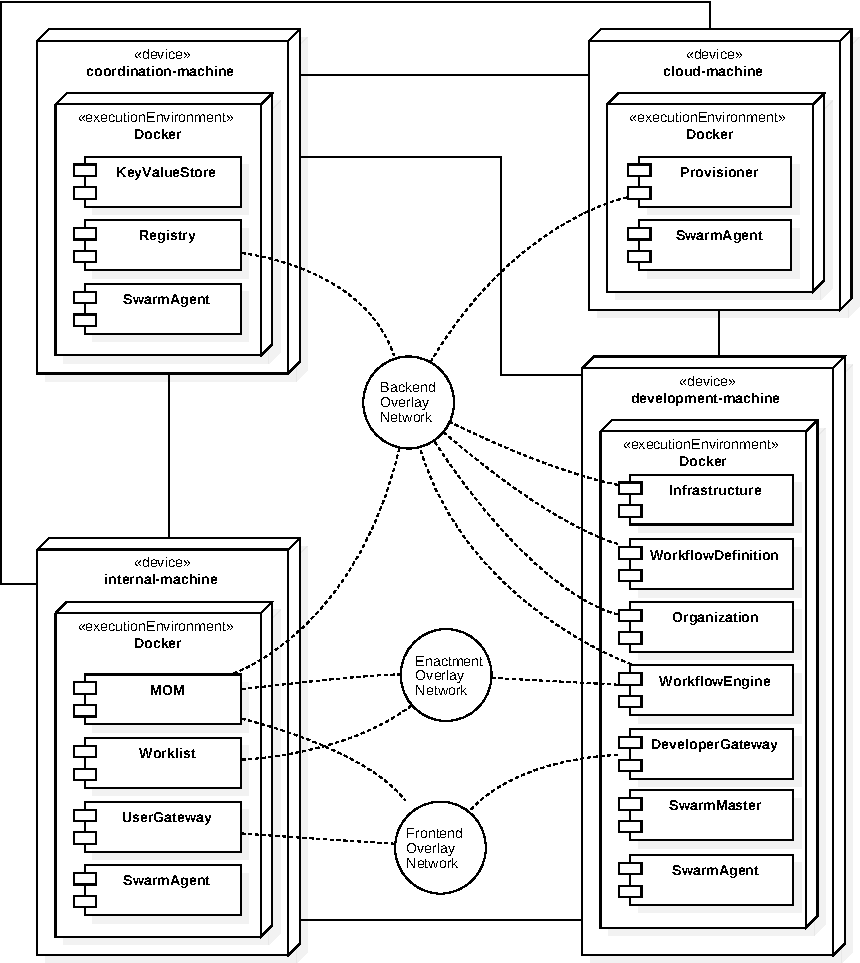
\includegraphics[width=0.95\textwidth]{content/images/deployment_diagram-crop.pdf}
    \caption*{\scriptsize Note: the depicted distribution of containers to nodes is just exemplarily. Most of them could run on any node in the swarm. The only mandatory assignments are the swarm agents, of which each node needs one, and the provisioners, of which each node that is intended to execute workflows on needs one. \\Also, the databases and their respective data volumes were omitted for the sake of clarity.}
    \caption{UML deployment diagram of the prototype}
    \label{fig:deployment_diagram_of_the_architecture}
  \end{figure}

  \begin{listing}[!htbp]
    \inputminted[lastline=47,fontsize=\footnotesize,linenos=true,numberblanklines=true,showspaces=false,breaklines=true,baselinestretch=1]{bash}{../code/_setup/setup_1_environment.sh}
    \caption{Setup of the machines for the exemplary deployment (1/2) }
  \label{lst:setup_exemplary_deployment_1}
  \end{listing}

  \begin{listing}[!htbp]
    \inputminted[firstline=48,fontsize=\footnotesize,linenos=true,numberblanklines=true,showspaces=false,breaklines=true,baselinestretch=1]{bash}{../code/_setup/setup_1_environment.sh}
    \caption{Setup of the machines for the exemplary deployment (2/2) }
  \label{lst:setup_exemplary_deployment_1_2}
  \end{listing}

  \begin{listing}[!htbp]
    \inputminted[firstline=48,fontsize=\footnotesize,linenos=true,numberblanklines=true,showspaces=false,breaklines=true,baselinestretch=1]{bash}{../code/_setup/setup_2_dev_services.sh}
    \caption{Setup of the services for the exemplary deployment }
  \label{lst:setup_exemplary_deployment_2}
  \end{listing}

  \begin{listing}[!htbp]
    \inputminted[lastline=50,fontsize=\footnotesize,linenos=true,numberblanklines=true,showspaces=false,breaklines=true,baselinestretch=1]{yaml}{../code/wfms.yml}
    \caption{Docker Compose file of the WfMS (1/5)}
  \label{lst:the_whole_docker_compose_file_1}
  \end{listing}

  \begin{listing}[!htbp]
    \inputminted[firstline=51,lastline=98,fontsize=\footnotesize,linenos=true,numberblanklines=true,showspaces=false,breaklines=true,baselinestretch=1]{yaml}{../code/wfms.yml}
    \caption{Docker Compose file of the WfMS (2/5)}
  \label{lst:the_whole_docker_compose_file_2}
  \end{listing}

  \begin{listing}[!htbp]
    \inputminted[firstline=99,lastline=145,fontsize=\footnotesize,linenos=true,numberblanklines=true,showspaces=false,breaklines=true,baselinestretch=1]{yaml}{../code/wfms.yml}
    \caption{Docker Compose file of the WfMS (3/5)}
  \label{lst:the_whole_docker_compose_file_3}
  \end{listing}

  \begin{listing}[!htbp]
    \inputminted[firstline=146,lastline=197,fontsize=\footnotesize,linenos=true,numberblanklines=true,showspaces=false,breaklines=true,baselinestretch=1]{yaml}{../code/wfms.yml}
    \caption{Docker Compose file of the WfMS (4/5)}
  \label{lst:the_whole_docker_compose_file_4}
  \end{listing}

  \begin{listing}[!htbp]
    \inputminted[firstline=198,fontsize=\footnotesize,linenos=true,numberblanklines=true,showspaces=false,breaklines=true,baselinestretch=1]{yaml}{../code/wfms.yml}
    \caption{Docker Compose file of the WfMS (5/5)}
  \label{lst:the_whole_docker_compose_file_5}
  \end{listing}

\clearpage
\AnhChapter{Case study}

  \begin{figure}[htbp]
    \centering
    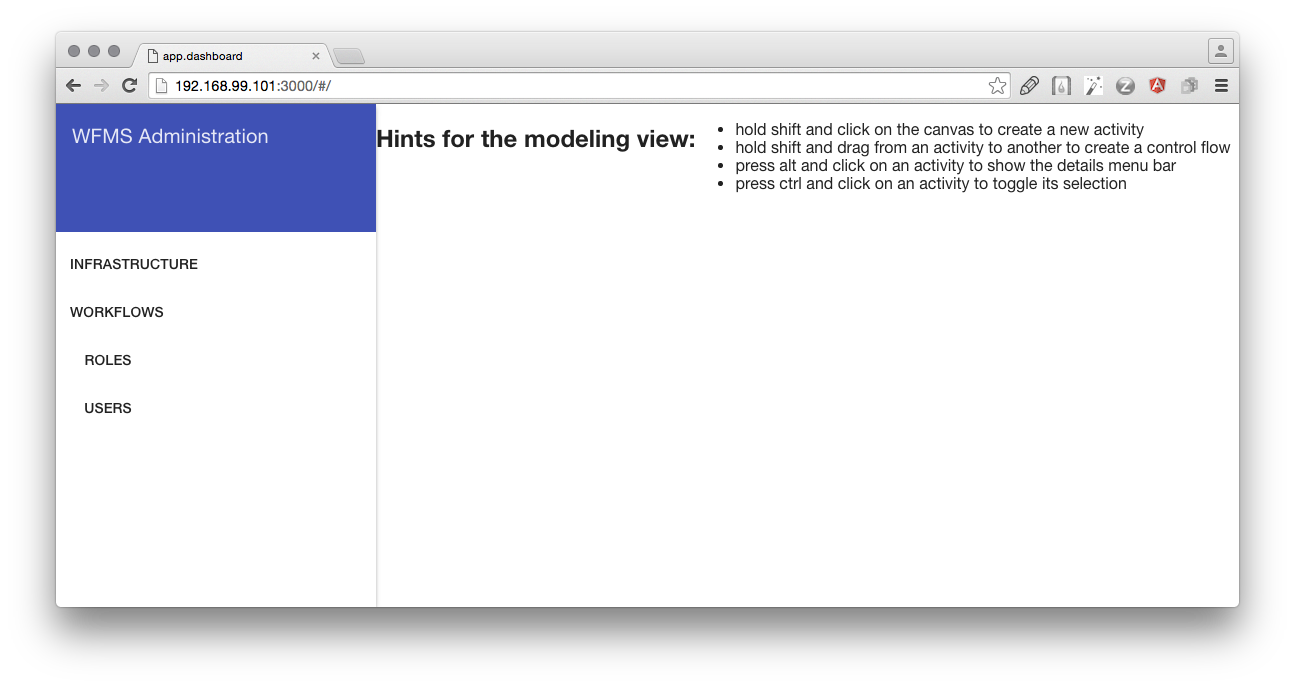
\includegraphics[width=\textwidth]{./content/images/usecase/case_study_6.png}
    \caption{Dashboard of the prototype}
    \label{fig:dashboard}
  \end{figure}

  \begin{figure}[htbp]
    \centering
    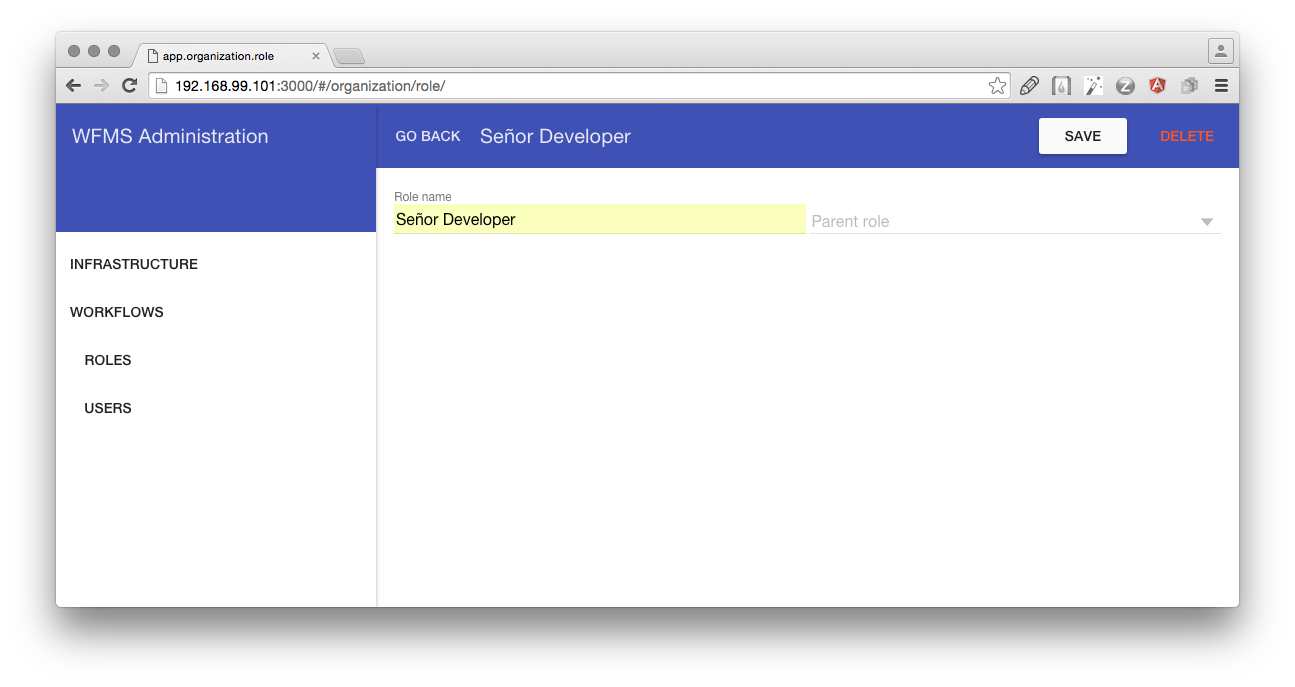
\includegraphics[width=\textwidth]{./content/images/usecase/case_study_8.png}
    \caption{Roles view of the prototype}
    \label{fig:dev_role}
  \end{figure}

  \begin{figure}[htbp]
    \centering
    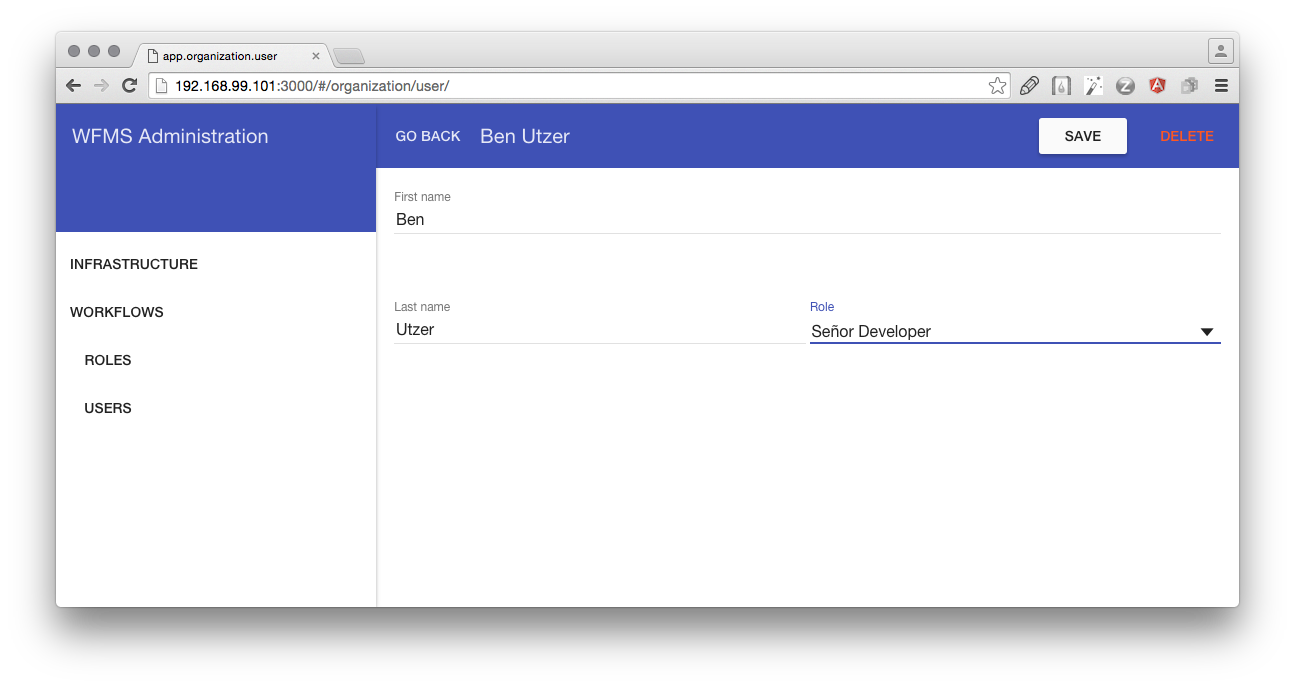
\includegraphics[width=\textwidth]{./content/images/usecase/case_study_9.png}
    \caption{Users view of the prototype}
    \label{fig:dev_user}
  \end{figure}

  \begin{figure}[htbp]
    \centering
    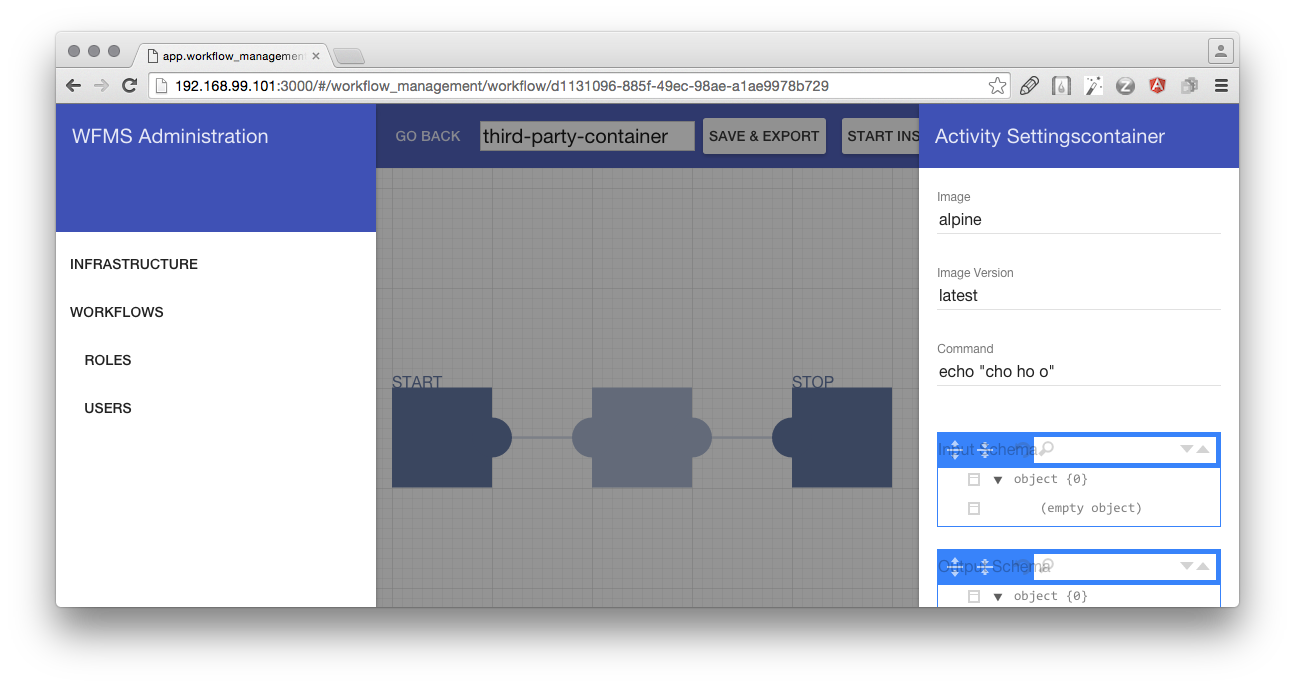
\includegraphics[width=\textwidth]{./content/images/usecase/case_study_10.png}
    \caption{Modeling a third party container workflow}
    \label{fig:tpc_wf}
  \end{figure}

  \begin{figure}[htbp]
    \centering
    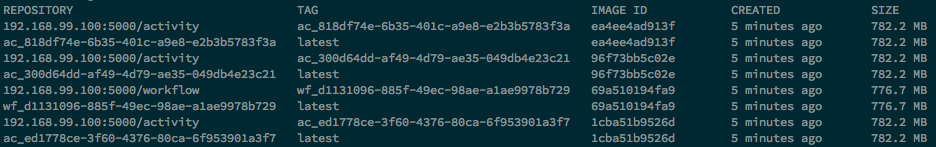
\includegraphics[width=\textwidth]{./content/images/usecase/case_study_12.png}
    \caption{Created images for the third party container workflow}
    \label{fig:tpc_images}
  \end{figure}

  \begin{figure}[htbp]
    \centering
    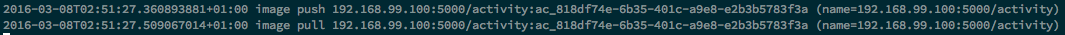
\includegraphics[width=\textwidth]{./content/images/usecase/case_study_13.png}
    \caption{Provisioner reacts to pushed image by initiating pull}
    \label{fig:provisioner_pulls}
  \end{figure}

  \begin{figure}[htbp]
    \centering
    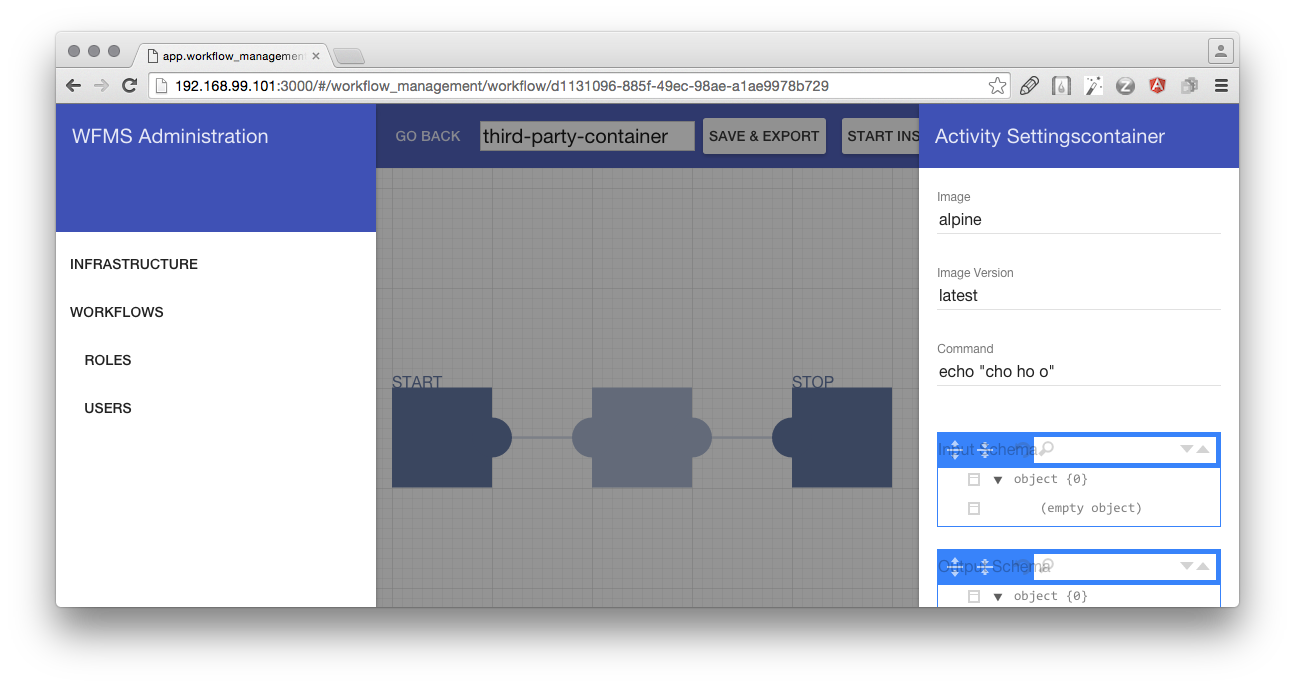
\includegraphics[width=\textwidth]{./content/images/usecase/case_study_10.png}
    \caption{Modeling a manual activity workflow}
    \label{fig:manual_wf}
  \end{figure}

  \begin{figure}[htbp]
    \centering
    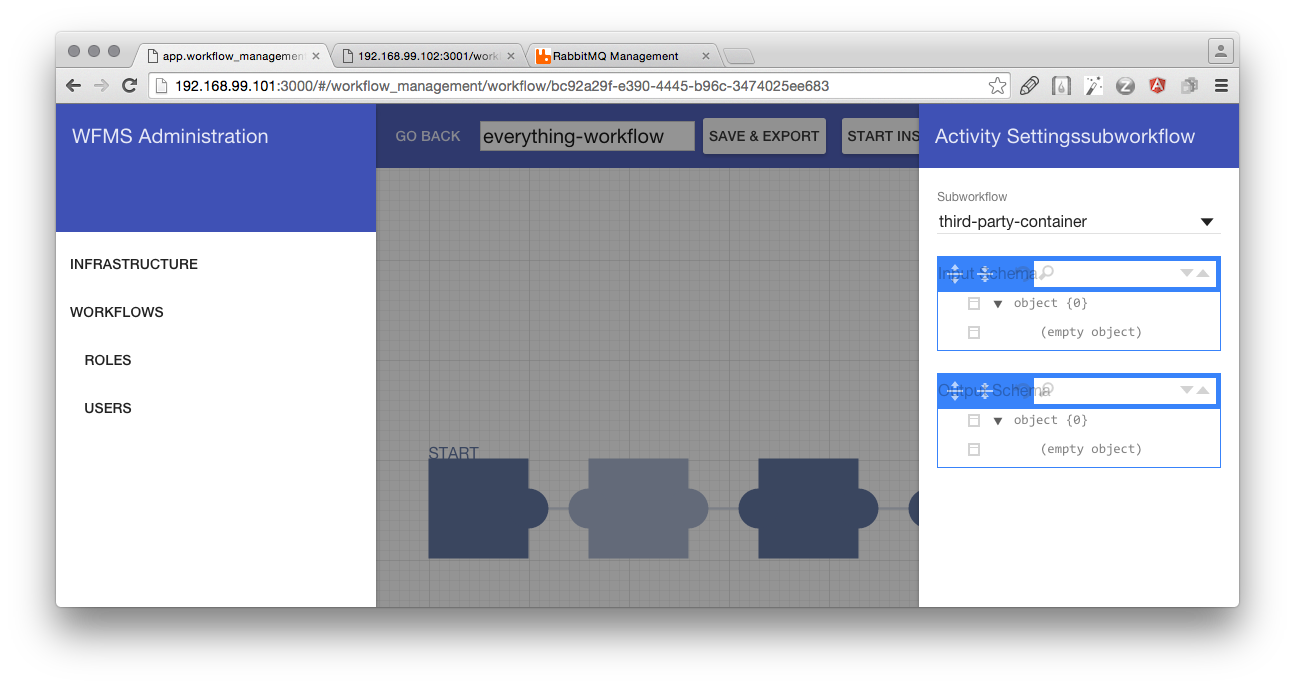
\includegraphics[width=\textwidth]{./content/images/usecase/case_study_26.png}
    \caption{Modeling a sub-workflow workflow}
    \label{fig:subwf_wf}
  \end{figure}

  \begin{figure}[htbp]
    \centering
    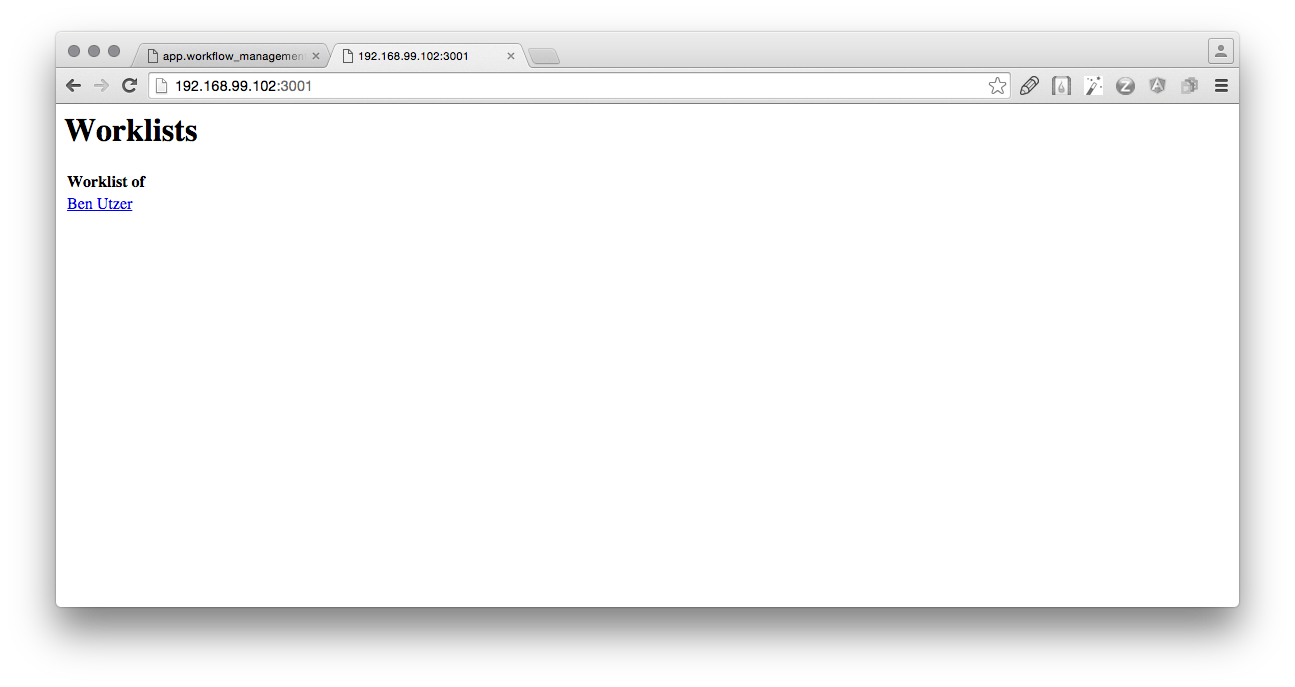
\includegraphics[width=\textwidth]{./content/images/usecase/case_study_19.png}
    \caption{Worklist overview in the user gateway}
    \label{fig:wl_index}
  \end{figure}

  \begin{figure}[htbp]
    \centering
    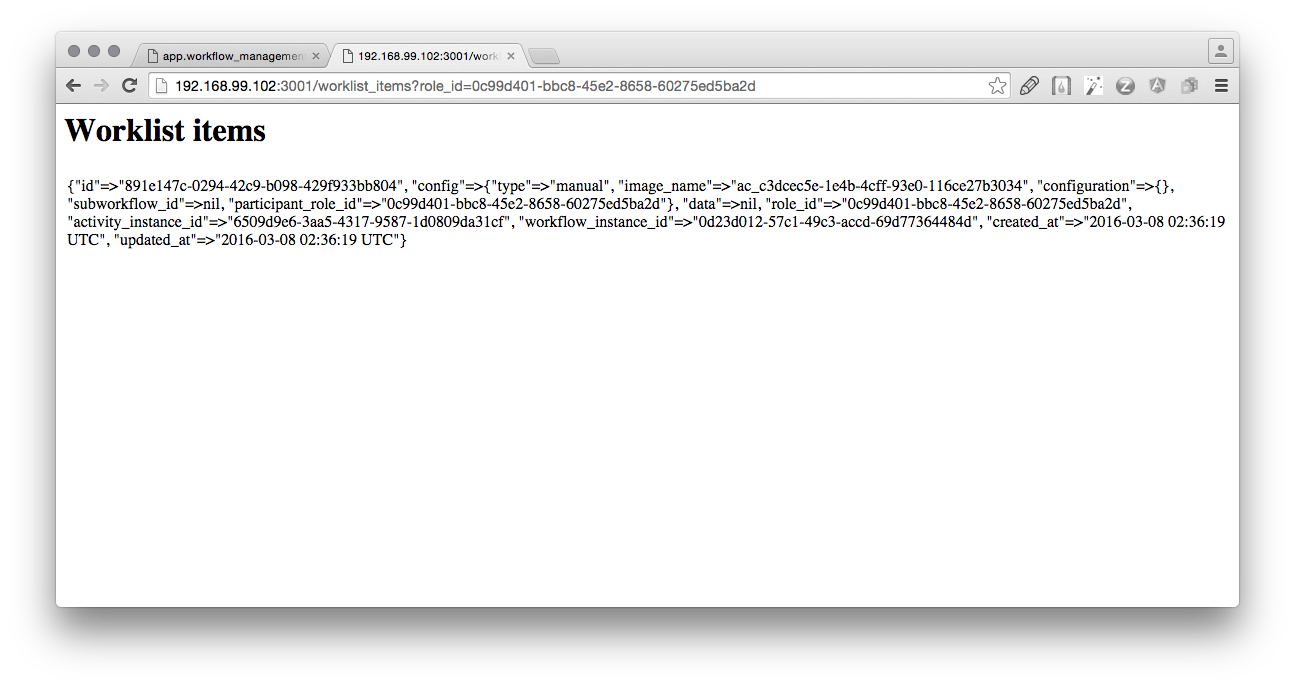
\includegraphics[width=\textwidth]{./content/images/usecase/case_study_20.png}
    \caption{Worklist item overview of a user in the user gateway}
    \label{fig:wl_user}
  \end{figure}

  \begin{figure}[htbp]
    \centering
    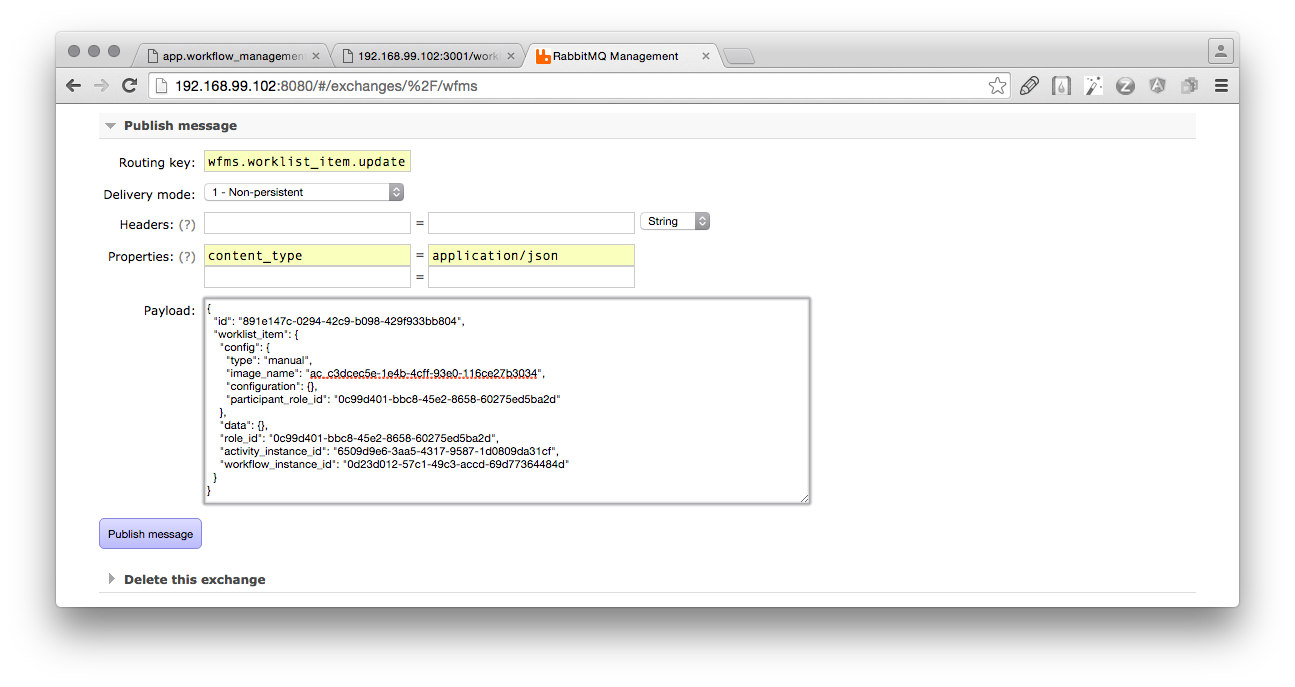
\includegraphics[width=\textwidth]{./content/images/usecase/case_study_22.png}
    \caption{Manually updating worklist item in RabbitMQ admin interface}
    \label{fig:wl_update}
  \end{figure}

  \begin{figure}[htbp]
    \centering
    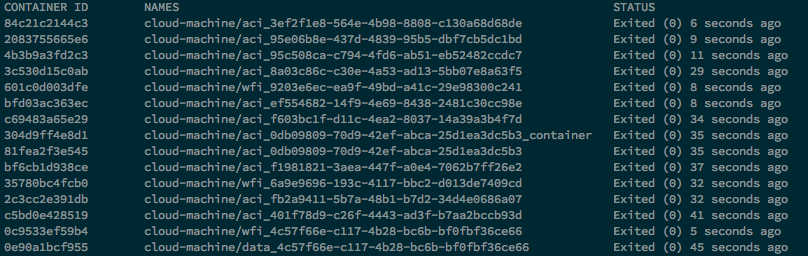
\includegraphics[width=\textwidth]{./content/images/usecase/case_study_25.png}
    \caption{Executed containers for the case study}
    \label{fig:exe_containers}
  \end{figure}

  \begin{figure}[htbp]
    \centering
    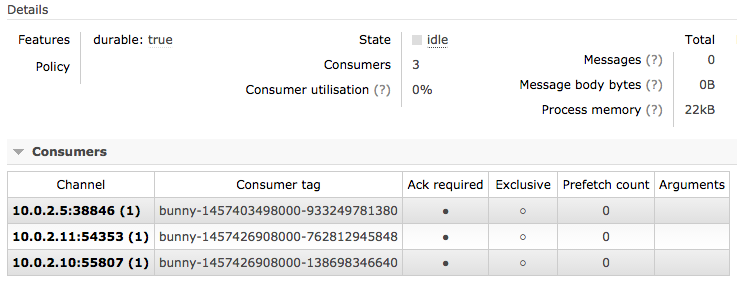
\includegraphics[width=\textwidth]{./content/images/usecase/case_study_27.png}
    \caption{Multiple engine instances subscribed to the same queue}
    \label{fig:mult_engines}
  \end{figure}

  \begin{figure}[htbp]
    \centering
    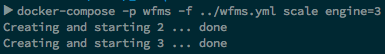
\includegraphics[width=\textwidth]{./content/images/usecase/case_study_28.png}
    \caption{Scaling up the engine service}
    \label{fig:mult_engines_2}
  \end{figure}

  % \begin{listing}[!h]
  %   \inputminted[fontsize=\footnotesize,linenos=true,numberblanklines=true,showspaces=false,breaklines=true,baselinestretch=1]{json}{./content/snippets/example_output_2.json}
  %   \caption*{Annotations are not part of the original output}
  %   \caption{Resulting data of the workflow enactment in the case study}
  % \label{lst:resulting_data_set}
  % \end{listing}


